\documentclass[]{article}
\usepackage{lmodern}
\usepackage{amssymb,amsmath}
\usepackage{ifxetex,ifluatex}
\usepackage{fixltx2e} % provides \textsubscript
\ifnum 0\ifxetex 1\fi\ifluatex 1\fi=0 % if pdftex
  \usepackage[T1]{fontenc}
  \usepackage[utf8]{inputenc}
\else % if luatex or xelatex
  \ifxetex
    \usepackage{mathspec}
  \else
    \usepackage{fontspec}
  \fi
  \defaultfontfeatures{Ligatures=TeX,Scale=MatchLowercase}
\fi
% use upquote if available, for straight quotes in verbatim environments
\IfFileExists{upquote.sty}{\usepackage{upquote}}{}
% use microtype if available
\IfFileExists{microtype.sty}{%
\usepackage{microtype}
\UseMicrotypeSet[protrusion]{basicmath} % disable protrusion for tt fonts
}{}
\usepackage[margin=1in]{geometry}
\usepackage{hyperref}
\hypersetup{unicode=true,
            pdftitle={Sparse covariance estimation},
            pdfauthor={Xuelong Wang},
            pdfborder={0 0 0},
            breaklinks=true}
\urlstyle{same}  % don't use monospace font for urls
\usepackage{graphicx,grffile}
\makeatletter
\def\maxwidth{\ifdim\Gin@nat@width>\linewidth\linewidth\else\Gin@nat@width\fi}
\def\maxheight{\ifdim\Gin@nat@height>\textheight\textheight\else\Gin@nat@height\fi}
\makeatother
% Scale images if necessary, so that they will not overflow the page
% margins by default, and it is still possible to overwrite the defaults
% using explicit options in \includegraphics[width, height, ...]{}
\setkeys{Gin}{width=\maxwidth,height=\maxheight,keepaspectratio}
\IfFileExists{parskip.sty}{%
\usepackage{parskip}
}{% else
\setlength{\parindent}{0pt}
\setlength{\parskip}{6pt plus 2pt minus 1pt}
}
\setlength{\emergencystretch}{3em}  % prevent overfull lines
\providecommand{\tightlist}{%
  \setlength{\itemsep}{0pt}\setlength{\parskip}{0pt}}
\setcounter{secnumdepth}{5}
% Redefines (sub)paragraphs to behave more like sections
\ifx\paragraph\undefined\else
\let\oldparagraph\paragraph
\renewcommand{\paragraph}[1]{\oldparagraph{#1}\mbox{}}
\fi
\ifx\subparagraph\undefined\else
\let\oldsubparagraph\subparagraph
\renewcommand{\subparagraph}[1]{\oldsubparagraph{#1}\mbox{}}
\fi

%%% Use protect on footnotes to avoid problems with footnotes in titles
\let\rmarkdownfootnote\footnote%
\def\footnote{\protect\rmarkdownfootnote}

%%% Change title format to be more compact
\usepackage{titling}

% Create subtitle command for use in maketitle
\providecommand{\subtitle}[1]{
  \posttitle{
    \begin{center}\large#1\end{center}
    }
}

\setlength{\droptitle}{-2em}

  \title{Sparse covariance estimation}
    \pretitle{\vspace{\droptitle}\centering\huge}
  \posttitle{\par}
    \author{Xuelong Wang}
    \preauthor{\centering\large\emph}
  \postauthor{\par}
      \predate{\centering\large\emph}
  \postdate{\par}
    \date{2019-12-25}

\usepackage{float,amsmath, bbm, siunitx, bm}
\usepackage{pdfpages}
\floatplacement{figure}{H}
\newcommand{\indep}{\rotatebox[origin=c]{90}{$\models$}}

\begin{document}
\maketitle

{
\setcounter{tocdepth}{2}
\tableofcontents
}
\section{Motivation}\label{motivation}

After decorrelation with the information of the historical data, the
correlation between the covariate is reduced. However, there are still
some correlation coeifficients are large. That may suggest that after
using the historical data, the decorrelated data still is not
uncorrelated. But the correlation structure becomes a sparse and
symmetric. Therefore, we could apply another decorrelation to further
reudce the non-zero correlation, so that we may have a better
performance on the following variance estimation procedure.

\section{Simulation}\label{simulation}

\subsection{Simulation procedure}\label{simulation-procedure}

\subsubsection{Standardization will not change total
variance}\label{standardization-will-not-change-total-variance}

\begin{enumerate}
\def\labelenumi{\arabic{enumi}.}
\tightlist
\item
  Standardize the X \(\tilde{Z}_m = (X-\mu)A_1\)
\item
  Generate the interaction based on the
  \(\tilde{Z}_{int} = \tilde{Z}_m*\tilde{Z}_m\) without the square terms
  and set \(\tilde{Z}_t = (\tilde{Z}_m, \tilde{Z}_{int})\)
\item
  Generate the Y based on the \(\tilde{Z}_t\)
\item
  Estimate the \(Var(\tilde{Z}_t \beta_t)\) by \(Z = \tilde{Z}_tA_2\),
  where \(A_2\) is for decorrelation
\end{enumerate}

Note that the \(Var(\tilde{Z}_t \beta_t) = Var(Z\gamma)\),
\(A_2 = \hat{\Sigma}^{-1/2}_h\) or
\(A_2 = \hat{\Sigma}^{-1/2}_h \hat{\Sigma}^{-1/2}_s\)

\subsection{Decorrelation steps}\label{decorrelation-steps}

\subsection{two steps decorrelation}\label{two-steps-decorrelation}

\begin{enumerate}
\def\labelenumi{\arabic{enumi}.}
\tightlist
\item
  Decorrelation by covariance matrix estimated by historical data
\item
  If after the step 1, the correlation is still large, then we may need
  a second decorrelation by sparse precision method
\end{enumerate}

\subsection{\texorpdfstring{Dpglasso:
\href{https://arxiv.org/pdf/1111.5479.pdf}{The Graphical Lasso: New
Insights and
Alternatives}}{Dpglasso: The Graphical Lasso: New Insights and Alternatives}}\label{dpglasso-the-graphical-lasso-new-insights-and-alternatives}

\begin{enumerate}
\def\labelenumi{\arabic{enumi}.}
\tightlist
\item
  An Alternatives for Glasso
\item
  Glasso works on \(W\) the covariance matrix, but its alg cannot make
  sure the precision matrix \(\Theta\) is positive definite.
\item
  Dpglasso can provide both \(W\) and \(\Theta\) be positive definite
\end{enumerate}

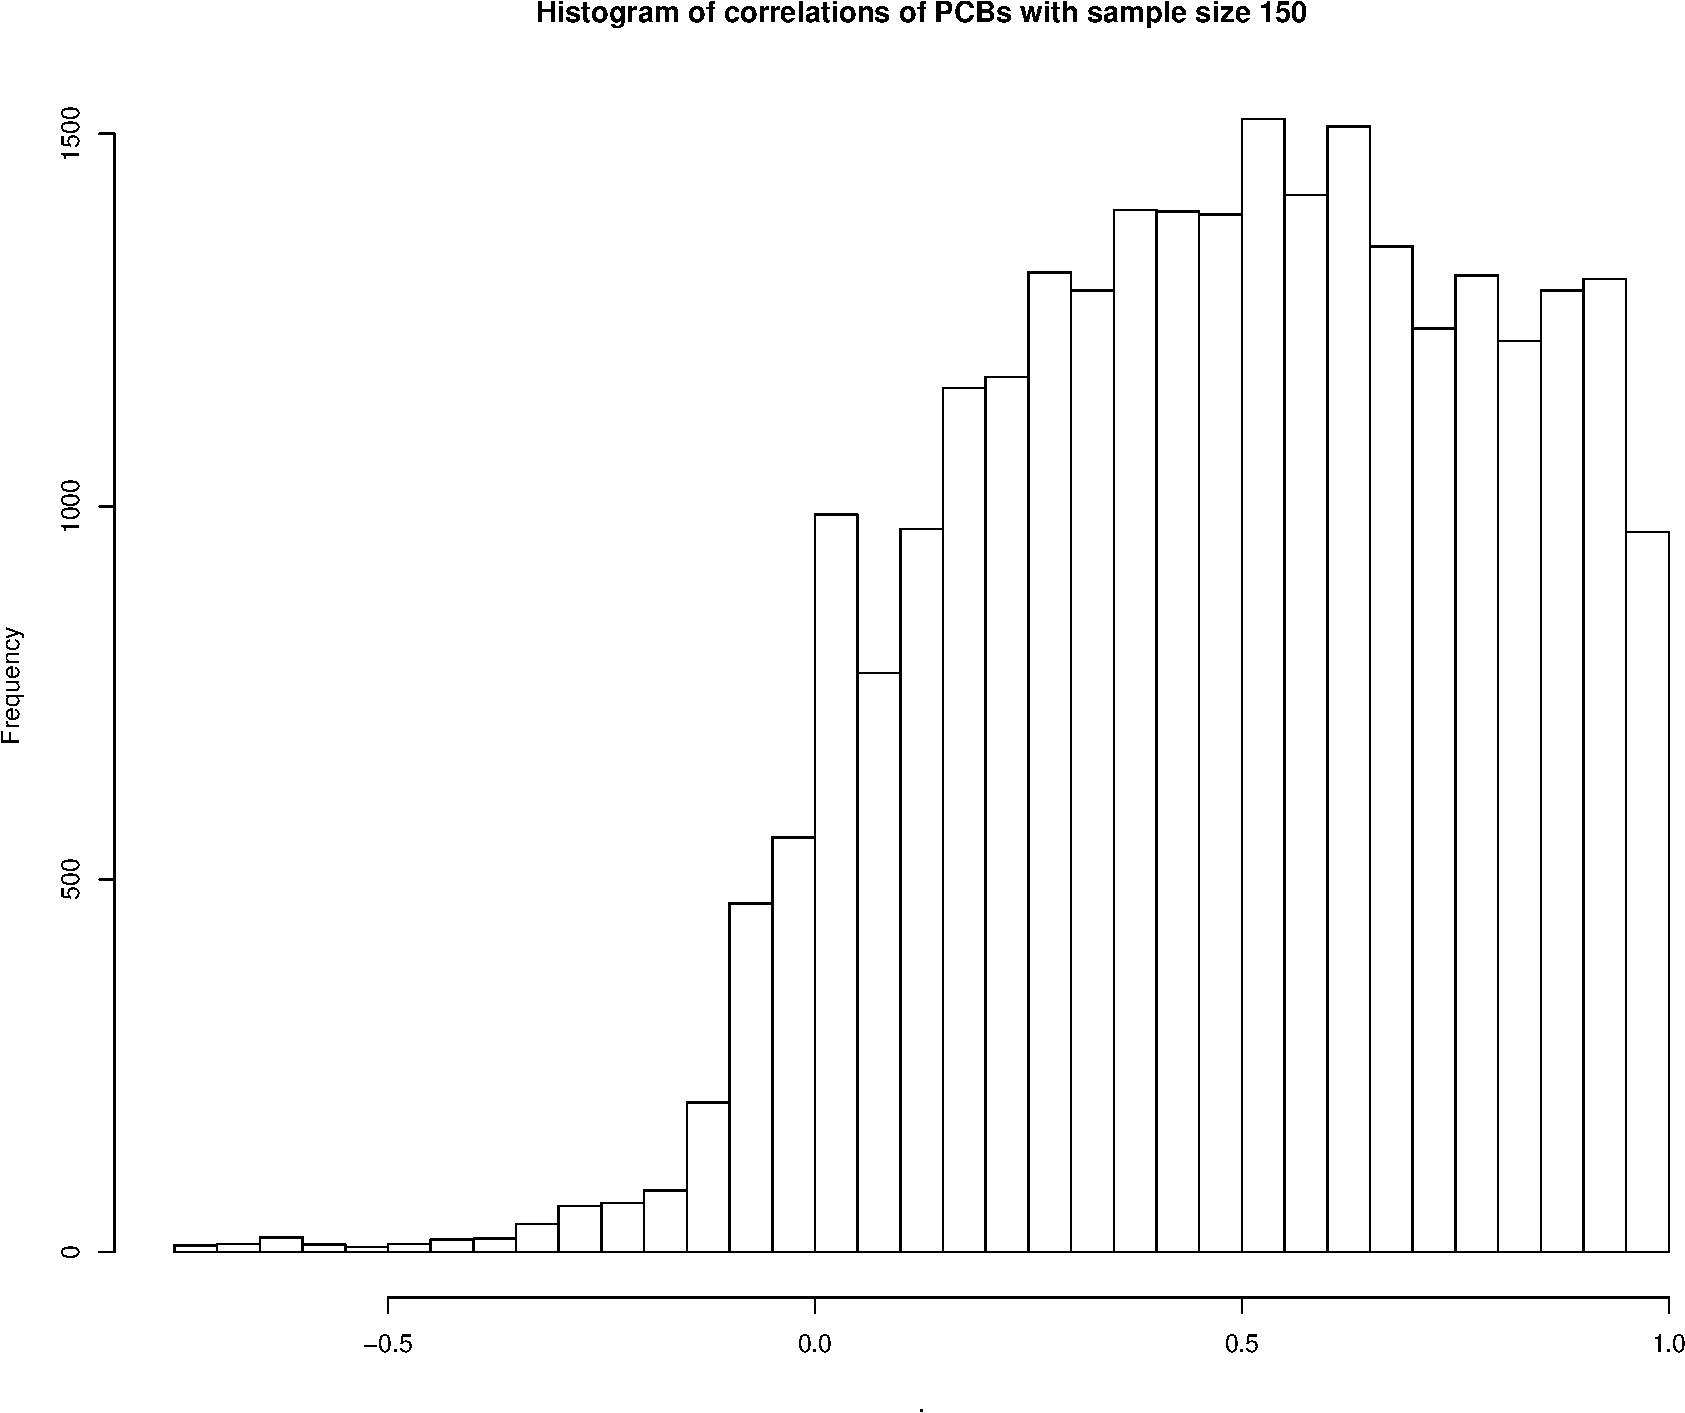
\includegraphics{Low_levels_covariance_sparse_decorr_files/figure-latex/unnamed-chunk-1-1.pdf}
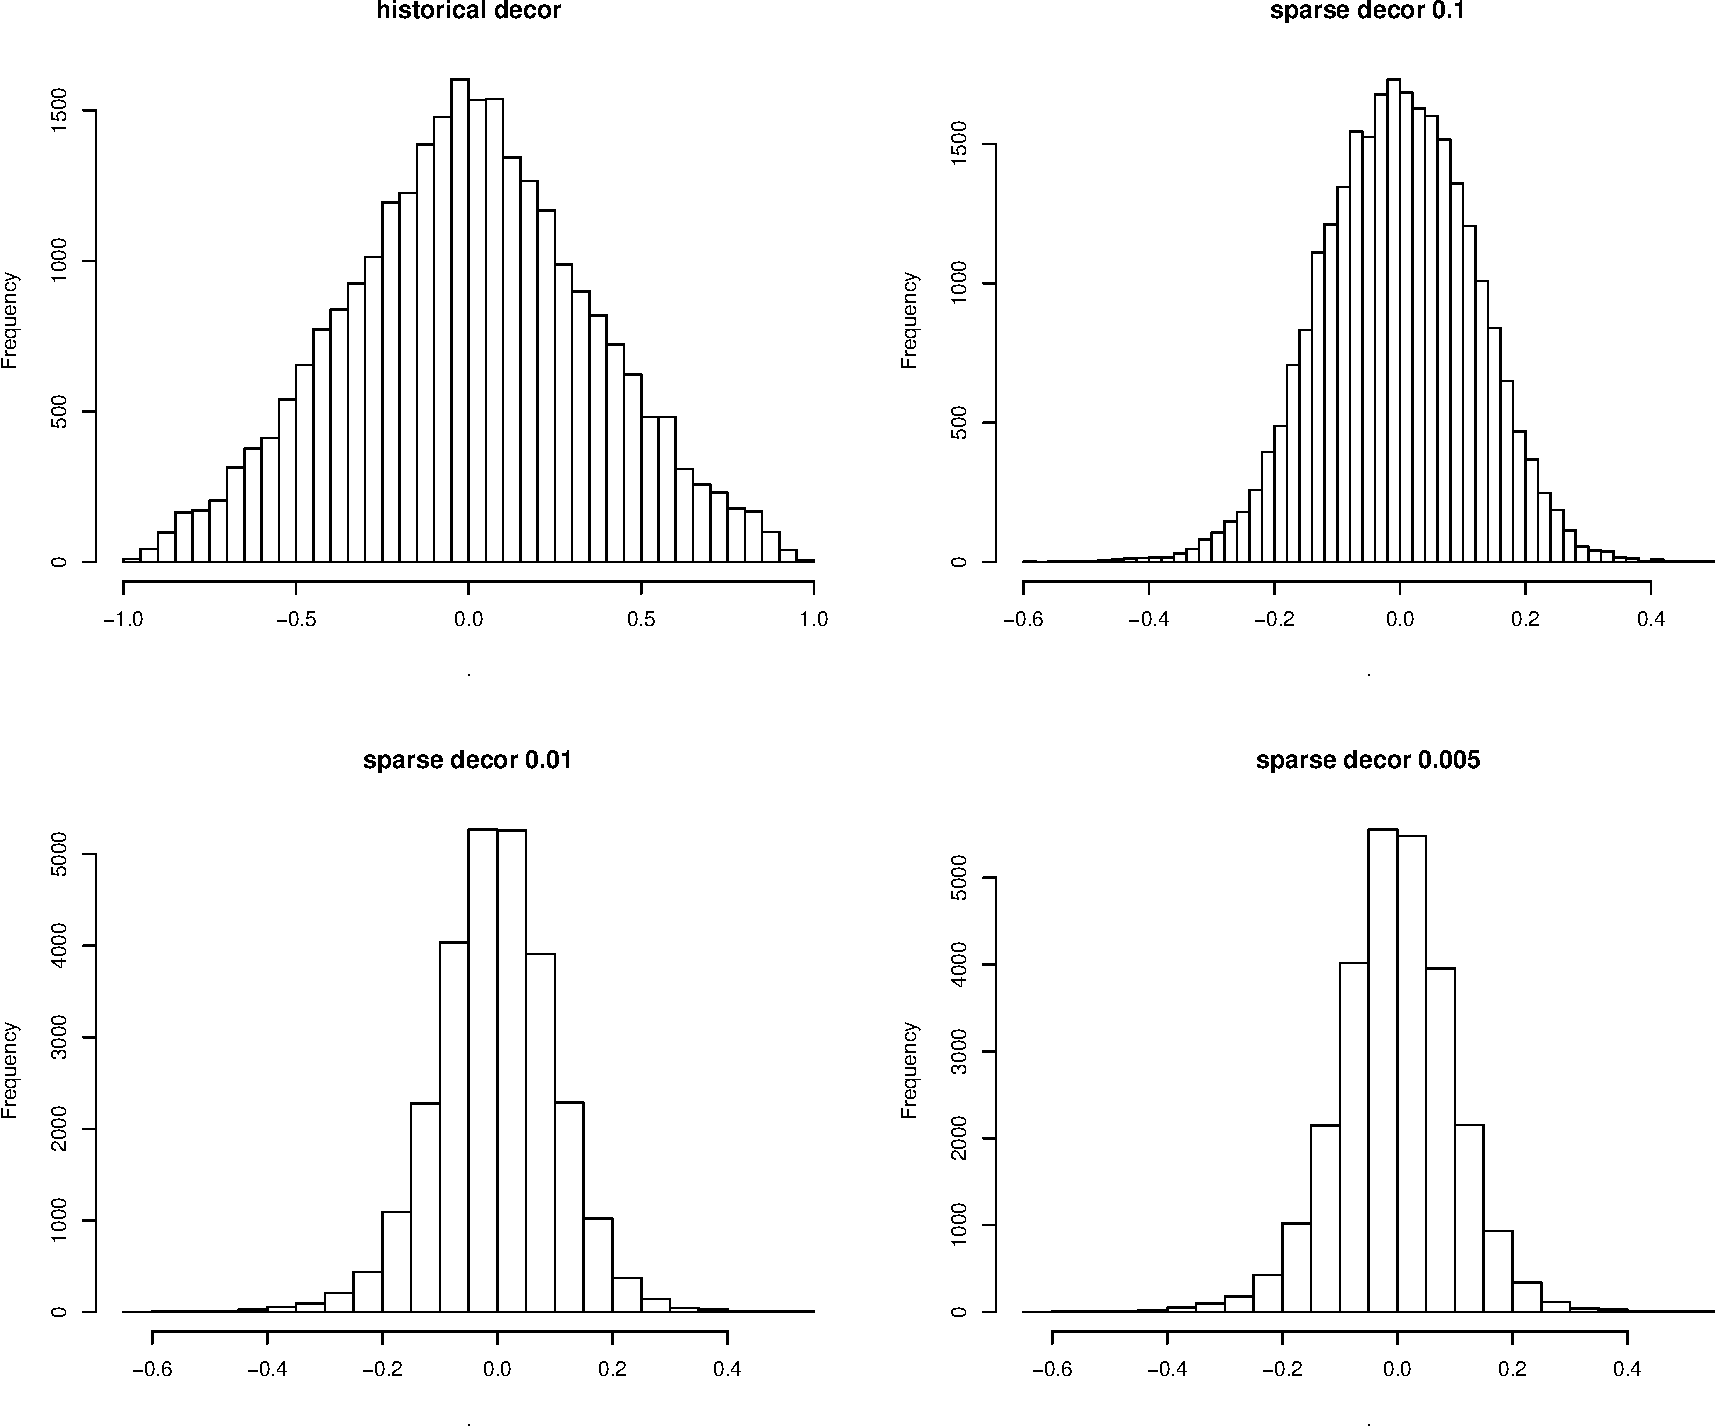
\includegraphics{Low_levels_covariance_sparse_decorr_files/figure-latex/unnamed-chunk-1-2.pdf}

\newpage

\subsection{PCB}\label{pcb}

\subsubsection{None}\label{none}

\begin{verbatim}
   var_main_effect var_inter_effect cov_main_inter_effect var_total_effect
1:               8                2                  0.62               11
   structure decor x_dist
1:        un FALSE   1999
\end{verbatim}

\begin{verbatim}
       n MSE est_var est_mean NA_total     method
 1:  100 206     112       21        3 EigenPrism
 2:  100 153     108       18        0       GCTA
 3:  150 304     112       25        0 EigenPrism
 4:  150 278     149       23        0       GCTA
 5:  231 276      83       25        0 EigenPrism
 6:  231 217      86       23        0       GCTA
 7:  500 NaN      NA      NaN      100 EigenPrism
 8:  500 472     166       29        0       GCTA
 9: 1000 NaN      NA      NaN      100 EigenPrism
10: 1000 495     113       31        0       GCTA
\end{verbatim}

\subsubsection{Hist}\label{hist}

\begin{verbatim}
   var_main_effect var_inter_effect cov_main_inter_effect var_total_effect
1:               8                2                  0.62               11
   structure decor x_dist
1:        un  TRUE   1999
\end{verbatim}

\begin{verbatim}
       n MSE est_var est_mean NA_total     method
 1:  100  31      32       11        3 EigenPrism
 2:  100  22      22       11        0       GCTA
 3:  150  26      26       11        0 EigenPrism
 4:  150  21      21       11        0       GCTA
 5:  231  19      20       11        0 EigenPrism
 6:  231  14      14       11        0       GCTA
 7:  500 NaN      NA      NaN      100 EigenPrism
 8:  500  31      31       12        0       GCTA
 9: 1000 NaN      NA      NaN      100 EigenPrism
10: 1000  44      39       13        1       GCTA
\end{verbatim}

\begin{verbatim}
   var_main_effect var_inter_effect cov_main_inter_effect var_total_effect
1:               8                2                  0.62               11
   structure decor x_dist
1:        un  TRUE   1999
\end{verbatim}

\begin{verbatim}
       n MSE est_var est_mean NA_total     method
 1:  100  31      32       11        3 EigenPrism
 2:  100  22      22       11        0       GCTA
 3:  150  26      26       11        0 EigenPrism
 4:  150  20      21       11        0       GCTA
 5:  231  19      20       11        0 EigenPrism
 6:  231  14      14       11        0       GCTA
 7:  500 NaN      NA      NaN      100 EigenPrism
 8:  500  31      31       12        0       GCTA
 9: 1000 NaN      NA      NaN      100 EigenPrism
10: 1000  44      39       13        0       GCTA
\end{verbatim}

\subsubsection{Hist + sparse}\label{hist-sparse}

\begin{verbatim}
   var_main_effect var_inter_effect cov_main_inter_effect var_total_effect
1:               8                2                  0.62               11
   structure decor x_dist
1:        un  TRUE   1999
\end{verbatim}

\begin{verbatim}
       n  MSE est_var est_mean NA_total     method
 1:  100 14.6   14.68     11.4        0 EigenPrism
 2:  100 14.0   14.11     11.2        0       GCTA
 3:  150  8.6    7.91     10.4        0 EigenPrism
 4:  150  6.9    6.78     10.8        0       GCTA
 5:  231 11.6    7.42      9.2        0 EigenPrism
 6:  231  5.2    4.37     10.3        0       GCTA
 7:  500  NaN      NA      NaN      100 EigenPrism
 8:  500  3.1    1.53     10.0        0       GCTA
 9: 1000  NaN      NA      NaN      100 EigenPrism
10: 1000  2.4    0.99     10.1        1       GCTA
\end{verbatim}

\begin{verbatim}
   var_main_effect var_inter_effect cov_main_inter_effect var_total_effect
1:               8                2                  0.62               11
   structure decor x_dist
1:        un  TRUE   1999
\end{verbatim}

\begin{verbatim}
       n  MSE est_var est_mean NA_total     method
 1:  100 14.6   14.68     11.4        0 EigenPrism
 2:  100 13.8   13.98     11.2        0       GCTA
 3:  150  8.6    7.91     10.4        0 EigenPrism
 4:  150  7.0    6.82     10.8        0       GCTA
 5:  231 11.6    7.42      9.2        0 EigenPrism
 6:  231  5.2    4.37     10.3        0       GCTA
 7:  500  NaN      NA      NaN      100 EigenPrism
 8:  500  3.1    1.53     10.0        0       GCTA
 9: 1000  NaN      NA      NaN      100 EigenPrism
10: 1000  2.3    0.99     10.1        0       GCTA
\end{verbatim}

\subsection{Chi}\label{chi}

\subsubsection{None}\label{none-1}

\begin{verbatim}
   var_main_effect var_inter_effect cov_main_inter_effect var_total_effect
1:               8                2                   1.8               14
   structure decor x_dist
1:        un FALSE    chi
\end{verbatim}

\begin{verbatim}
      n MSE est_var est_mean NA_total     method
1:  100 108      67       20        3 EigenPrism
2:  100  77      68       17        0       GCTA
3:  200 213      90       25        7 EigenPrism
4:  200 189     109       23        0       GCTA
5:  500 NaN      NA      NaN      100 EigenPrism
6:  500 131      31       24        0       GCTA
7: 1000 NaN      NA      NaN      100 EigenPrism
8: 1000 134      20       24        0       GCTA
\end{verbatim}

\subsubsection{hist}\label{hist-1}

\begin{verbatim}
   var_main_effect var_inter_effect cov_main_inter_effect var_total_effect
1:               8                2                   1.8               14
   structure decor x_dist
1:        un  TRUE    chi
\end{verbatim}

\begin{verbatim}
      n  MSE est_var est_mean NA_total     method
1:  100 23.4    21.5       12        0 EigenPrism
2:  100 18.5    16.5       12        0       GCTA
3:  200 15.5    12.9       12        0 EigenPrism
4:  200  9.3     8.2       13        0       GCTA
5:  500  NaN      NA      NaN      100 EigenPrism
6:  500  4.1     2.8       13        0       GCTA
7: 1000  NaN      NA      NaN      100 EigenPrism
8: 1000  3.0     1.3       12        1       GCTA
\end{verbatim}

\begin{verbatim}
   var_main_effect var_inter_effect cov_main_inter_effect var_total_effect
1:               8                2                   1.8               14
   structure decor x_dist
1:        un  TRUE    chi
\end{verbatim}

\begin{verbatim}
      n  MSE est_var est_mean NA_total     method
1:  100 23.4    21.5       12        0 EigenPrism
2:  100 35.5    35.9       14        0       GCTA
3:  200 15.5    12.9       12        0 EigenPrism
4:  200 19.1    19.3       14        0       GCTA
5:  500  NaN      NA      NaN      100 EigenPrism
6:  500  5.2     4.7       13        0       GCTA
7: 1000  NaN      NA      NaN      100 EigenPrism
8: 1000  3.8     2.4       13        0       GCTA
\end{verbatim}

\subsubsection{hist + sparse}\label{hist-sparse-1}

\begin{verbatim}
   var_main_effect var_inter_effect cov_main_inter_effect var_total_effect
1:               8                2                   1.8               14
   structure decor x_dist
1:        un  TRUE    chi
\end{verbatim}

\begin{verbatim}
      n  MSE est_var est_mean NA_total     method
1:  100 27.7    27.6       14        0 EigenPrism
2:  100 26.9    27.1       14        0       GCTA
3:  200 12.4    10.7       12        0 EigenPrism
4:  200  8.9     8.8       13        0       GCTA
5:  500  NaN      NA      NaN      100 EigenPrism
6:  500  4.5     2.5       12        0       GCTA
7: 1000  NaN      NA      NaN      100 EigenPrism
8: 1000  4.1     1.8       12        0       GCTA
\end{verbatim}

\section{Mimic the histrocial covariance
situation}\label{mimic-the-histrocial-covariance-situation}

Based on the previous simulation, we found that if the historical data
is from extact the same distribution, then the sparse decorrelation may
not be neccessary. That is after doing the second step of decorrelation
the variance estimation does not get much improvement. So to mimic the
situation situation we change the simulation so that there is historical
covariance is not perfect.

\subsection{Simulation setup}\label{simulation-setup}

\begin{itemize}
\tightlist
\item
  \(p = 21\)
\item
  \(X \sim \chi^2_1\)
\item
  \(Cor(X)\) is the sample covariance of subset of standardized PCB data
  with \(n = 150\)\\
\item
  \(X_h = XB\), where
  \(B = \begin{bmatrix} 1 & 1 & 1 & 1 &1\dots \\ 0 & 1& 1& 1& 1\dots\\ 0& & 1 & 1 & 1\dots\\ 0& & & 1& 1\dots\\ 0& & & & 1\dots \end{bmatrix}\).
  So that the \(X_h\) is a column transfromation of \(X\), therefore the
  its covariance is different from the true value.
\end{itemize}

\subsection{Decorrelation result}\label{decorrelation-result}

\subsubsection{\texorpdfstring{\(X_h = X\)}{X\_h = X}}\label{x_h-x}

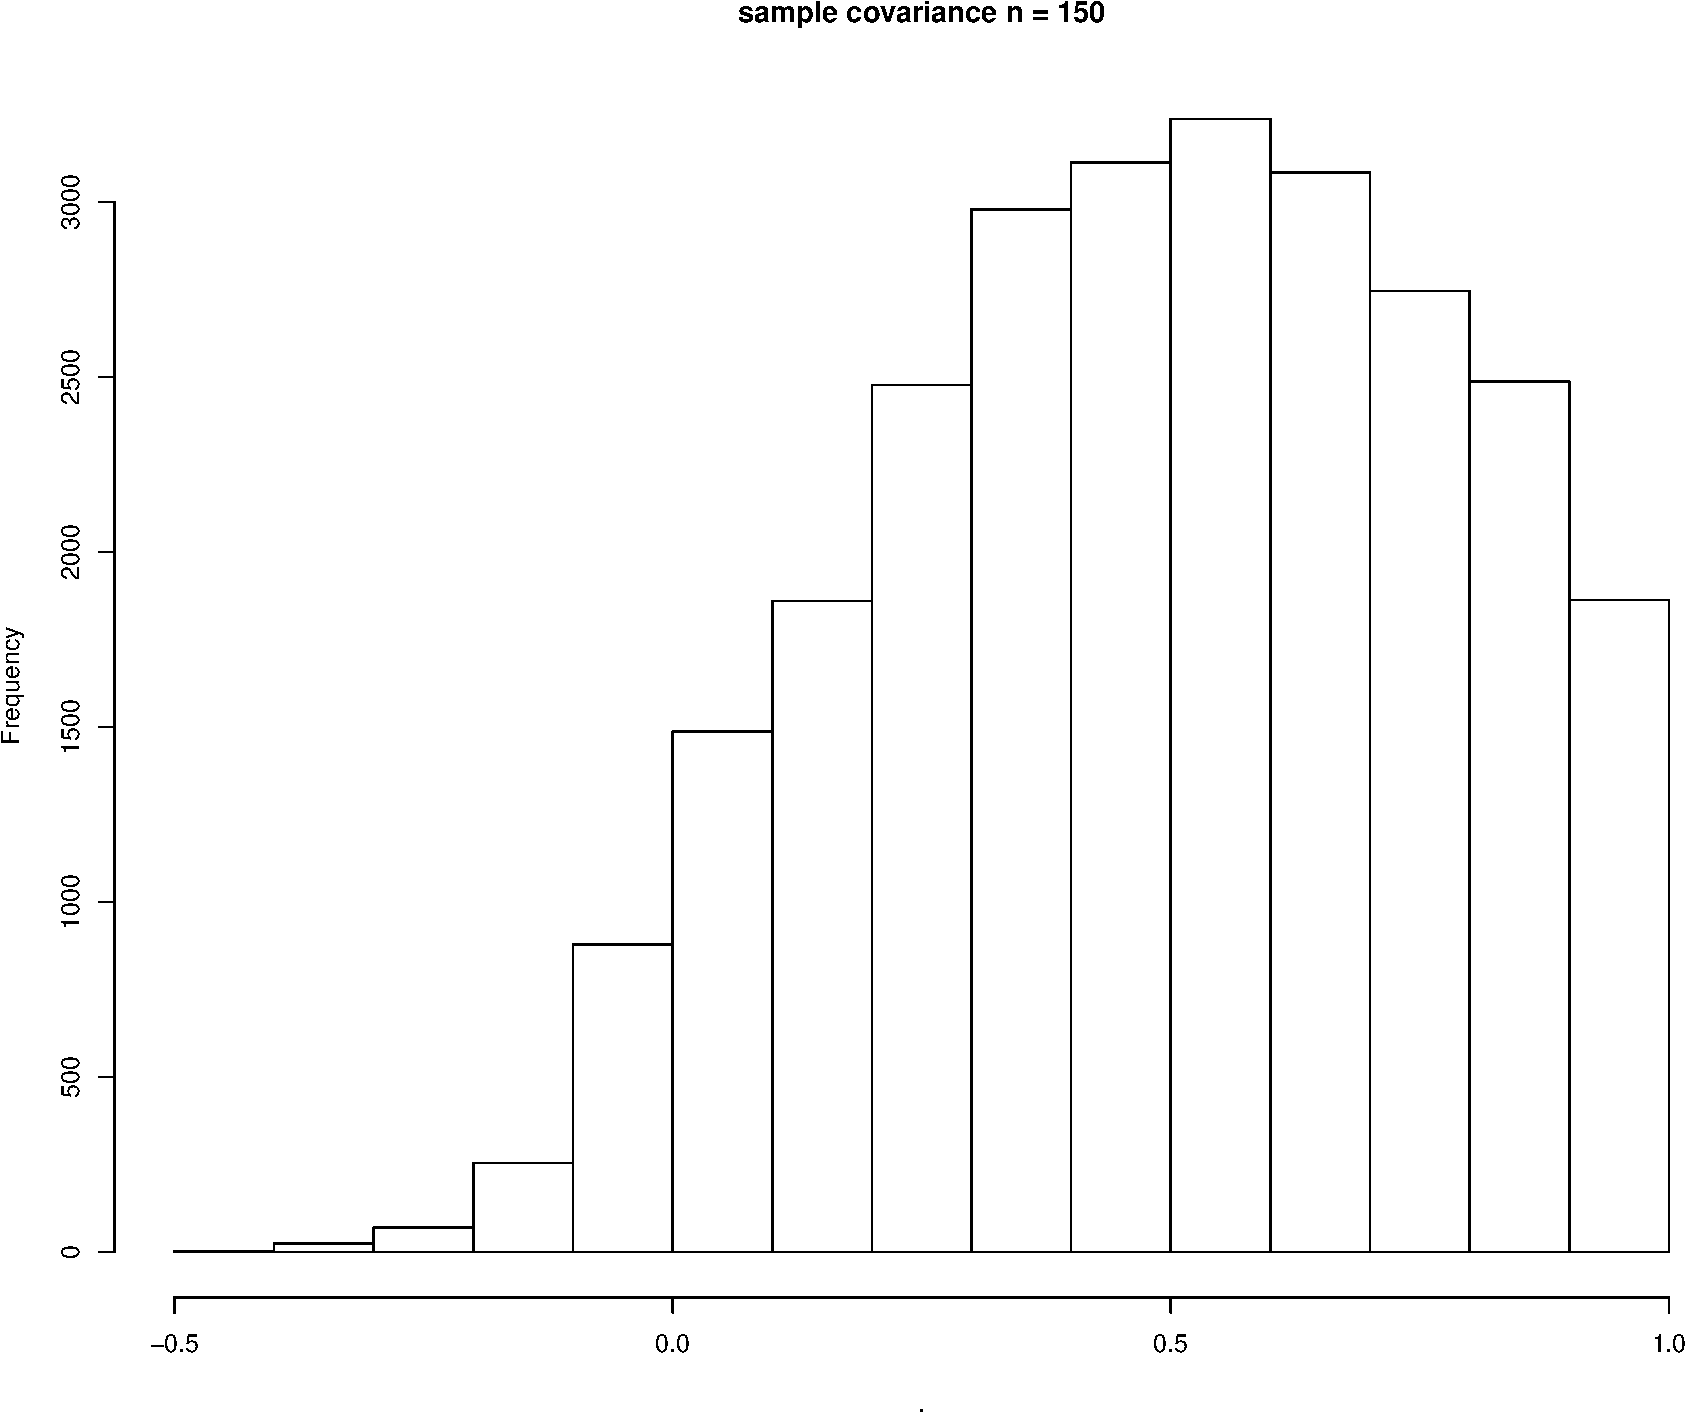
\includegraphics{Low_levels_covariance_sparse_decorr_files/figure-latex/unnamed-chunk-2-1.pdf}

\begin{verbatim}
   Min. 1st Qu.  Median    Mean 3rd Qu.    Max. 
  -0.42    0.29    0.50    0.49    0.72    1.00 
\end{verbatim}

\begin{verbatim}
   Min. 1st Qu.  Median    Mean 3rd Qu.    Max. 
  -0.96   -0.11    0.00    0.00    0.11    0.94 
\end{verbatim}

\begin{verbatim}
   Min. 1st Qu.  Median    Mean 3rd Qu.    Max. 
  -0.37   -0.06    0.00    0.00    0.06    0.48 
\end{verbatim}

\begin{verbatim}
   Min. 1st Qu.  Median    Mean 3rd Qu.    Max. 
  -0.33   -0.05    0.00    0.00    0.04    0.54 
\end{verbatim}

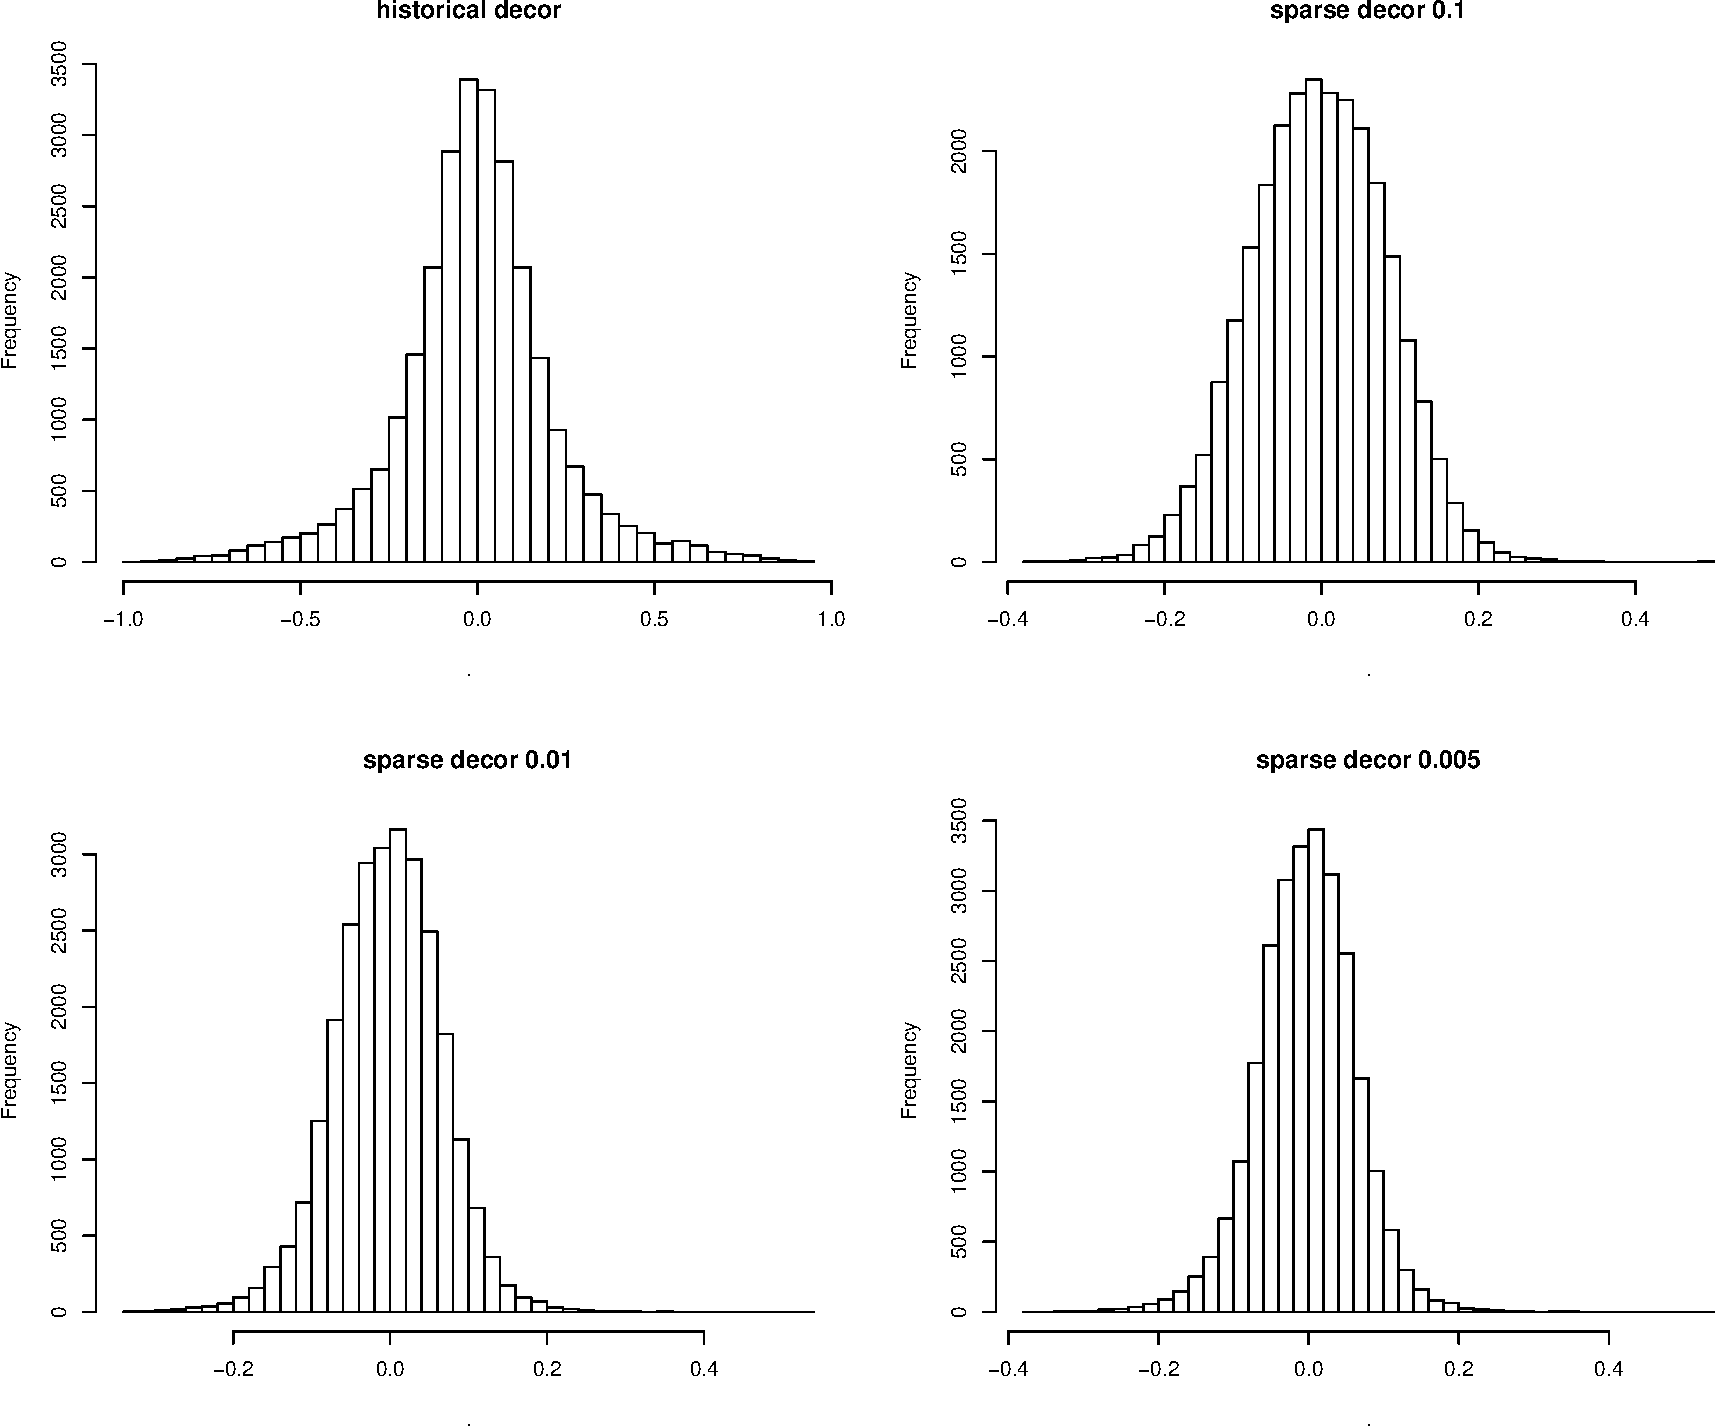
\includegraphics{Low_levels_covariance_sparse_decorr_files/figure-latex/unnamed-chunk-2-2.pdf}

\begin{verbatim}
   Min. 1st Qu.  Median    Mean 3rd Qu.    Max. 
  -0.37   -0.04    0.00    0.00    0.04    0.53 
\end{verbatim}

\subsubsection{\texorpdfstring{\(X_h = XB, t = 8\)}{X\_h = XB, t = 8}}\label{x_h-xb-t-8}

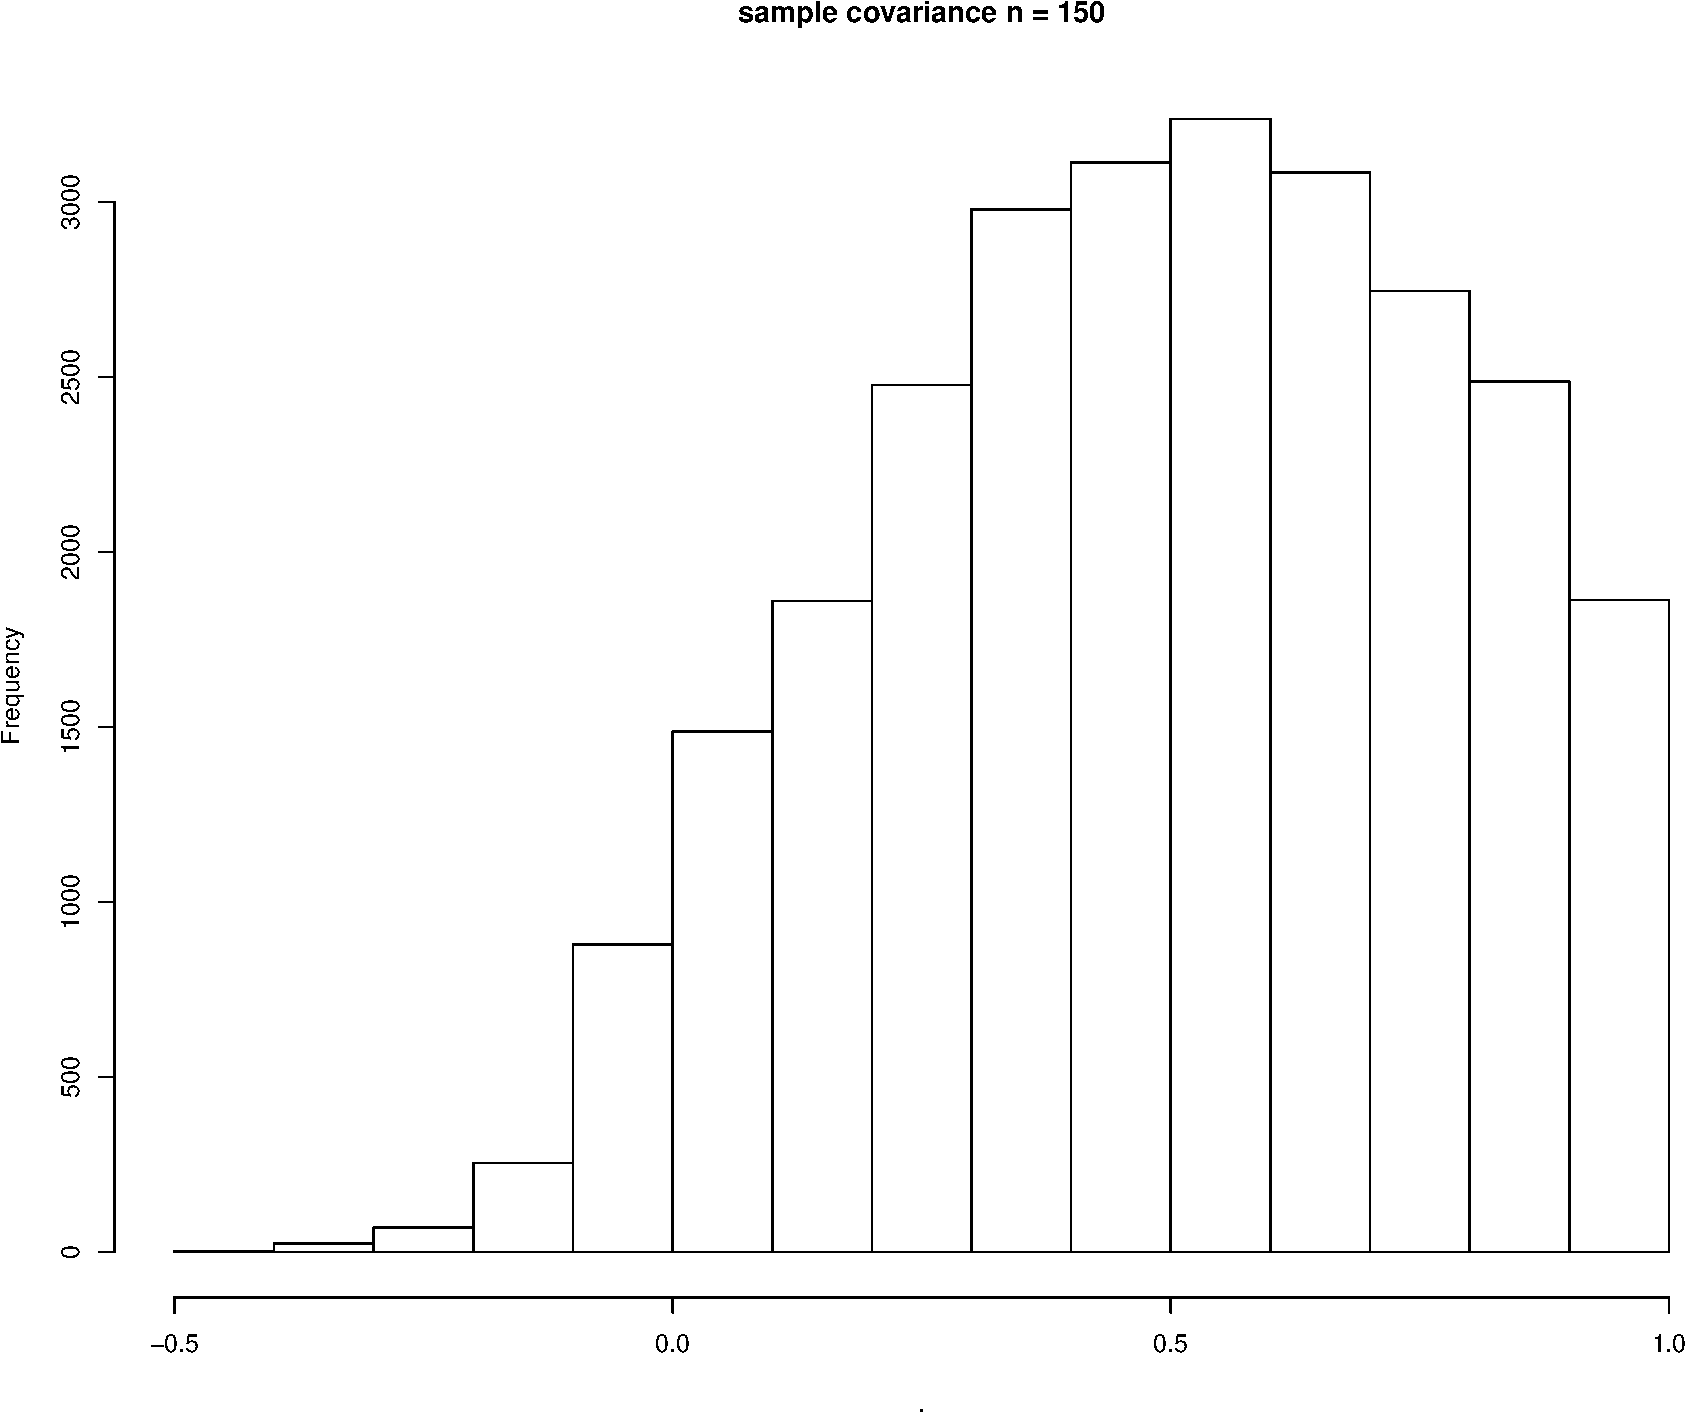
\includegraphics{Low_levels_covariance_sparse_decorr_files/figure-latex/unnamed-chunk-3-1.pdf}

\begin{verbatim}
   Min. 1st Qu.  Median    Mean 3rd Qu.    Max. 
  -0.42    0.29    0.50    0.49    0.72    1.00 
\end{verbatim}

\begin{verbatim}
   Min. 1st Qu.  Median    Mean 3rd Qu.    Max. 
  -0.93   -0.15    0.00    0.00    0.15    0.91 
\end{verbatim}

\begin{verbatim}
   Min. 1st Qu.  Median    Mean 3rd Qu.    Max. 
  -0.65   -0.04    0.00    0.00    0.04    0.42 
\end{verbatim}

\begin{verbatim}
   Min. 1st Qu.  Median    Mean 3rd Qu.    Max. 
  -0.64   -0.04    0.00    0.00    0.04    0.44 
\end{verbatim}

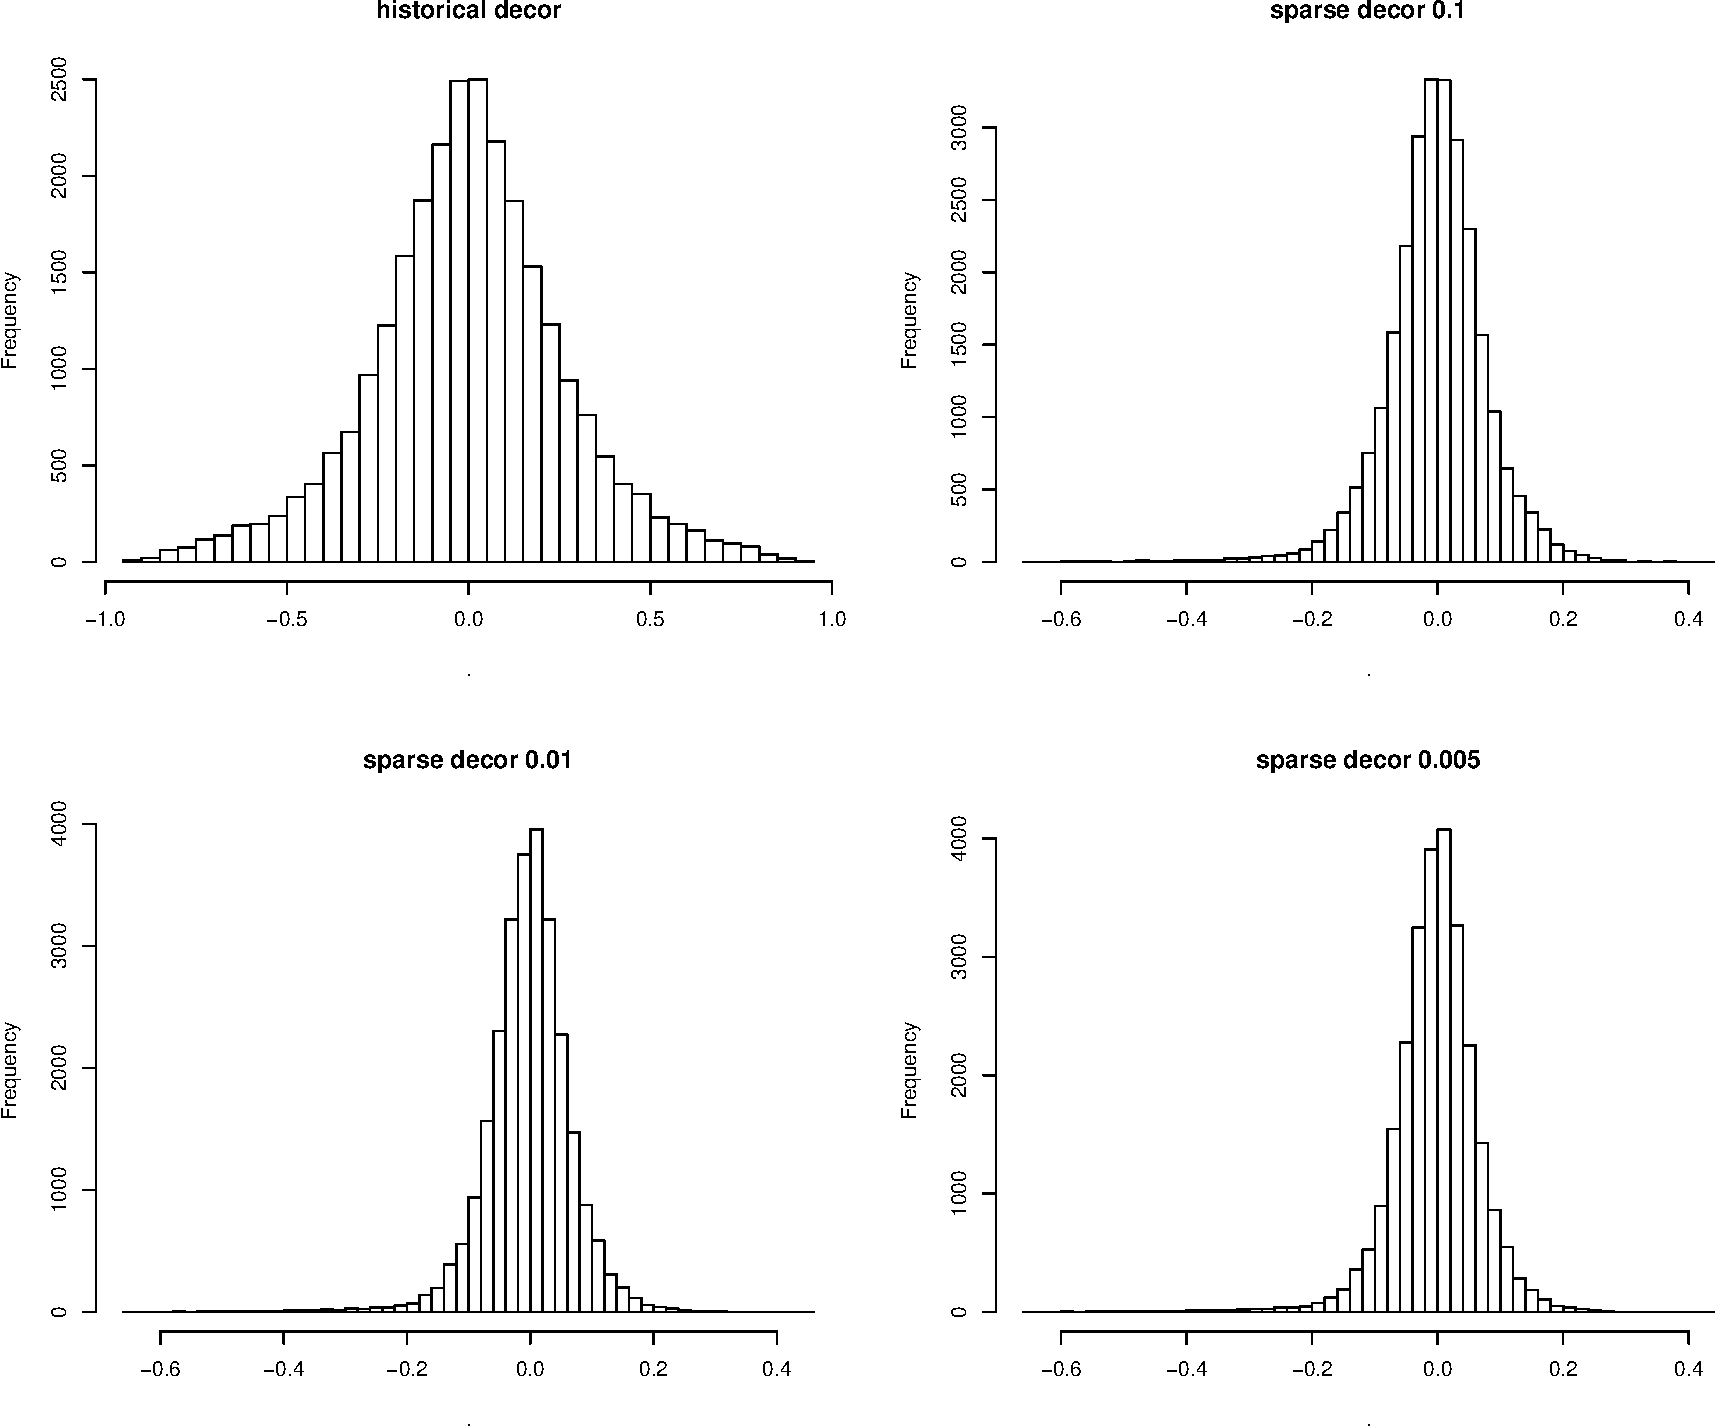
\includegraphics{Low_levels_covariance_sparse_decorr_files/figure-latex/unnamed-chunk-3-2.pdf}

\begin{verbatim}
   Min. 1st Qu.  Median    Mean 3rd Qu.    Max. 
  -0.64   -0.04    0.00    0.00    0.03    0.44 
\end{verbatim}

\subsection{Simulation result on the variance estimation
process}\label{simulation-result-on-the-variance-estimation-process}

\subsubsection{None}\label{none-2}

\begin{verbatim}
   var_main_effect var_inter_effect cov_main_inter_effect var_total_effect
1:               8                2                   1.8               14
   structure decor x_dist
1:        un FALSE    chi
\end{verbatim}

\begin{verbatim}
      n MSE est_var est_mean NA_total     method
1:  100 108      67       20        3 EigenPrism
2:  100  77      68       17        0       GCTA
3:  200 213      90       25        7 EigenPrism
4:  200 189     109       23        0       GCTA
5:  500 NaN      NA      NaN      100 EigenPrism
6:  500 131      31       24        0       GCTA
7: 1000 NaN      NA      NaN      100 EigenPrism
8: 1000 134      20       24        0       GCTA
\end{verbatim}

\subsubsection{Hist}\label{hist-2}

\begin{verbatim}
   var_main_effect var_inter_effect cov_main_inter_effect var_total_effect
1:               8                2                   1.8               14
   structure decor x_dist
1:        un  TRUE    chi
\end{verbatim}

\begin{verbatim}
      n MSE est_var est_mean NA_total     method
1:  100  32    27.3       11        0 EigenPrism
2:  100  25    18.1       11        0       GCTA
3:  200  29    22.8       11        0 EigenPrism
4:  200  19    13.4       11        0       GCTA
5:  500 NaN      NA      NaN      100 EigenPrism
6:  500  14     3.5       10        0       GCTA
7: 1000 NaN      NA      NaN      100 EigenPrism
8: 1000  15     2.9       10        0       GCTA
\end{verbatim}

\subsubsection{Hist + Sparse(0.1)}\label{hist-sparse0.1}

\begin{verbatim}
   var_main_effect var_inter_effect cov_main_inter_effect var_total_effect
1:               8                2                   1.8               14
   structure decor x_dist
1:        un  TRUE    chi
\end{verbatim}

\begin{verbatim}
      n  MSE est_var est_mean NA_total     method
1:  100 19.8    20.0       14        0 EigenPrism
2:  100 22.0    22.0       13        0       GCTA
3:  200 13.6     8.5       11        0 EigenPrism
4:  200  7.7     6.9       13        0       GCTA
5:  500  NaN      NA      NaN      100 EigenPrism
6:  500  6.0     1.5       12        0       GCTA
7: 1000  NaN      NA      NaN      100 EigenPrism
8: 1000 10.1     0.9       11        1       GCTA
\end{verbatim}

\subsubsection{Hist + Sparse(0.01)}\label{hist-sparse0.01}

\begin{verbatim}
   var_main_effect var_inter_effect cov_main_inter_effect var_total_effect
1:               8                2                   1.8               14
   structure decor x_dist
1:        un  TRUE    chi
\end{verbatim}

\begin{verbatim}
      n  MSE est_var est_mean NA_total     method
1:  100 39.5   39.37       14        0 EigenPrism
2:  100 22.5   22.69       13        0       GCTA
3:  200 13.7    8.43       11        0 EigenPrism
4:  200  7.5    6.19       13        0       GCTA
5:  500  NaN      NA      NaN      100 EigenPrism
6:  500  7.5    1.43       11        0       GCTA
7: 1000  NaN      NA      NaN      100 EigenPrism
8: 1000 10.6    0.93       11        1       GCTA
\end{verbatim}

\subsubsection{Hist + Sparse(0.001)}\label{hist-sparse0.001}

\begin{verbatim}
   var_main_effect var_inter_effect cov_main_inter_effect var_total_effect
1:               8                2                   1.8               14
   structure decor x_dist
1:        un  TRUE    chi
\end{verbatim}

\begin{verbatim}
      n  MSE est_var est_mean NA_total     method
1:  100 74.2   67.14       16        0 EigenPrism
2:  100 32.0   32.36       14        0       GCTA
3:  200 12.5    8.37       12        0 EigenPrism
4:  200  7.4    6.25       13        0       GCTA
5:  500  NaN      NA      NaN      100 EigenPrism
6:  500  7.7    1.43       11        0       GCTA
7: 1000  NaN      NA      NaN      100 EigenPrism
8: 1000 10.4    0.96       11        0       GCTA
\end{verbatim}

\subsubsection{Perfect Hist}\label{perfect-hist}

\begin{verbatim}
   var_main_effect var_inter_effect cov_main_inter_effect var_total_effect
1:               8                2                   1.8               14
   structure decor x_dist
1:        un  TRUE    chi
\end{verbatim}

\begin{verbatim}
      n  MSE est_var est_mean NA_total     method
1:  100 23.4    21.5       12        0 EigenPrism
2:  100 18.5    16.5       12        0       GCTA
3:  200 15.5    12.9       12        0 EigenPrism
4:  200  9.3     8.2       13        0       GCTA
5:  500  NaN      NA      NaN      100 EigenPrism
6:  500  4.1     2.8       13        0       GCTA
7: 1000  NaN      NA      NaN      100 EigenPrism
8: 1000  3.0     1.3       12        1       GCTA
\end{verbatim}

\subsubsection{Perfect Hist + Sparse(0.1)}\label{perfect-hist-sparse0.1}

\begin{verbatim}
   var_main_effect var_inter_effect cov_main_inter_effect var_total_effect
1:               8                2                   1.8               14
   structure decor x_dist
1:        un  TRUE    chi
\end{verbatim}

\begin{verbatim}
      n  MSE est_var est_mean NA_total     method
1:  100 27.7    27.6       14        0 EigenPrism
2:  100 26.9    27.1       14        0       GCTA
3:  200 12.4    10.7       12        0 EigenPrism
4:  200  8.9     8.8       13        0       GCTA
5:  500  NaN      NA      NaN      100 EigenPrism
6:  500  4.5     2.5       12        0       GCTA
7: 1000  NaN      NA      NaN      100 EigenPrism
8: 1000  4.1     1.8       12        0       GCTA
\end{verbatim}

\subsubsection{Perfect Hist +
Sparse(0.01)}\label{perfect-hist-sparse0.01}

\begin{verbatim}
   var_main_effect var_inter_effect cov_main_inter_effect var_total_effect
1:               8                2                   1.8               14
   structure decor x_dist
1:        un  TRUE    chi
\end{verbatim}

\begin{verbatim}
      n  MSE est_var est_mean NA_total     method
1:  100 59.9    54.4       11        3 EigenPrism
2:  100 60.5    59.7       13        0       GCTA
3:  200 13.6    13.0       15        0 EigenPrism
4:  200 12.4    12.4       14        0       GCTA
5:  500  NaN      NA      NaN      100 EigenPrism
6:  500  3.6     3.1       13        0       GCTA
7: 1000  NaN      NA      NaN      100 EigenPrism
8: 1000  2.9     2.1       13        0       GCTA
\end{verbatim}

\subsubsection{Perfect Hist +
Sparse(0.001)}\label{perfect-hist-sparse0.001}

\begin{verbatim}
   var_main_effect var_inter_effect cov_main_inter_effect var_total_effect
1:               8                2                   1.8               14
   structure decor x_dist
1:        un  TRUE    chi
\end{verbatim}

\begin{verbatim}
      n   MSE est_var est_mean NA_total     method
1:  100 148.2   146.6       15        0 EigenPrism
2:  100  76.4    76.7       13        0       GCTA
3:  200  32.2    27.3       16        3 EigenPrism
4:  200  12.5    12.4       14        0       GCTA
5:  500   NaN      NA      NaN      100 EigenPrism
6:  500   3.8     3.1       13        0       GCTA
7: 1000   NaN      NA      NaN      100 EigenPrism
8: 1000   2.7     2.4       13        0       GCTA
\end{verbatim}


\end{document}
